%%% Template originaly created by Karol Kozioł (mail@karol-koziol.net) and modified for ShareLaTeX use

\documentclass[11pt]{article}

\usepackage[T1]{fontenc}
\usepackage[utf8]{inputenc}
\usepackage{graphicx}
\usepackage{xcolor}
\usepackage{float}
\usepackage{tgtermes}
%\usepackage{natbib}
%\usepackage[subnum]{cases}
\usepackage[super]{nth}
%\bibpunct{(}{)}{;}{a}{}{,}
\usepackage{amsmath,amssymb}
\usepackage{enumerate}
\usepackage{multicol}
\usepackage{tikz}
\usepackage[amssymb]{SIunits}
\usepackage{rotating}
\usepackage{enumitem}
\usepackage{geometry}
\geometry{total={8.5in,11in},
left=1in,right=1in,%
bindingoffset=0mm, top=1in,bottom=1in}
\usepackage[super]{nth}
\usepackage[
pdftitle={Project 1}, 
pdfauthor={Jeremy Gibbs, University of Utah},
colorlinks=true,linkcolor=blue,urlcolor=blue,citecolor=blue,bookmarks=true,
bookmarksopenlevel=2]{hyperref}

\linespread{1.1}
\setlength{\parskip}{1em}
\setlength{\parindent}{0pt}
\newcommand{\linia}{\rule{\linewidth}{0.5pt}}

\makeatletter
\renewcommand{\maketitle}{
\begin{center}
\vspace{2ex}
{\huge \textsc{\@title}}
\vspace{1ex}
\\
\linia\\
ME EN 7710 \hfill Project \#1 \hfill Due Feb 9, 23\\
Modeling the Urban Surface Energy Balance
\vspace{4ex}
\end{center}
}
\makeatother
%%%

% custom footers and headers
\usepackage{fancyhdr,lastpage}
\pagestyle{fancy}
\lhead{}
\chead{}
\rhead{}
%\lfoot{Assignment \textnumero{} 5}
\cfoot{}
\rfoot{Page \thepage~/~\pageref*{LastPage}}
\renewcommand{\headrulewidth}{0pt}
\renewcommand{\footrulewidth}{0pt}
%

%%%----------%%%----------%%%----------%%%----------%%%

\begin{document}
\bibliographystyle{abbrv}
\title{Environmental Fluid Dynamics}

\maketitle
\vspace{-20pt}
\paragraph{\large Overview}~\\
The goal of this project is to obtain a working understanding of the Surface Energy Balance (SEB) for urban areas. For this project, you will model the urban SEB for a tower located in a suburban neighborhood in the Salt Lake Valley (Murray, UT) using the so-called LUMPS (Local-scale Urban Meteorological Parameterization Scheme) model. At the end of the project you will have a working simulation tool. 

\paragraph{\large Part I: Radiation Modeling (due: Feb 9)}~\\\\
Familiarize yourself with the LUMPS model by reading Grimmond and Oke (2002). Write and validate a sub-module to determining the net radiation balance. Using the equations presented in class, in the handouts and in the textbook, write a computer program to do the following: calculate the incoming direct beam solar radiation at any point in the northern hemisphere, at any time of the day, at any latitude ($\phi$), and for sloping terrain (slope angle $\hat\beta$ and slope azimuth $\hat \Omega$).  In doing this, assume the atmosphere has a net transmissivity that can modeled using the parameterization given in the provided handout for low, middle, and high cloud cover fractions or using a more advance model that you might find in the literature. Please hand in your computer code as well as answering the questions below.

\begin{enumerate}
	\item Determine the incoming solar radiation on a segment of horizontally homogeneous unobstructed flat terrain in Salt Lake City, UT on September 21, 2002 at 2 pm local time with no cloud cover (use the airport coordinates: $\phi=40.788^\circ$ North and $\lambda_e = 111.978^\circ$ West).
	\item For the same latitude, generate a contour plot of incoming solar radiation as a function of time of day and slope angle for (a) a north-facing slope ($\hat \Omega = 0$) on December 21 and (b) a south-facing ($\hat \Omega= 180$) slope on June 21.
	\item Determine the incoming solar radiation for the same day and time as in problem 1, for a slope on the Oquirrh mountains (assume $\hat \beta = 5^\circ$ and $\hat \Omega = 90^\circ$)
	\item Determine the incoming solar radiation for the same day and time as in problem 1, along the Wasatch front (assume $\hat \beta = 20^\circ$ and $\hat \Omega = 270^\circ$)
	\item Compare to supplied incoming solar radiation data from the Dugway Proving Grounds ($\hat \beta = 0$; $\phi = 40.142^\circ$ North and $\lambda_e = 113.267^\circ$ West). Note that the time series is in UTC +6 hours. Please use July 19, 2001.
	\item Compare to supplied incoming solar radiation data from the BLLAST experiment in Lannemezan, France ($\hat \beta = 0$;$\phi = 46^\circ 6' 32.9''$ North and $\lambda_e = 0^\circ 21' 32.1''$ East). Note that the time series given on the website for this is in UTC. Please use June 25, 2011.
\end{enumerate}

\paragraph{\large Part II: LUMPS Model and Evaluation (due: Feb 23)}
\begin{itemize}
\item Write the code for the LUMPS model and integrate the net radiation module from Part I into the LUMPS model.
\item Utilize the provided surface cover and morphometry data as well as basic meteorological data from the flux tower in Murray to calculate the full SEB.
\item Compare the calculated sensible and latent heat fluxes to those actually measured in the field. Note: you will get full diurnal solutions.
\item Please present your results in the form of a well-written AMS conference paper that includes a brief introduction and methods section. Use the Grimmond and Oke (2002) paper as a model. Your paper should be limited to 7 pages
\end{itemize}

\noindent This project should be done individually, but cooperation amongst students is encouraged.

\noindent Part I of the project report is due by \underline{Tuesday February \nth{7}} and Part II of the project is due by \underline{Tuesday February \nth{21}}.  Please contact me with any questions or problems.

\paragraph{\large Land Surface Cover Data}~\\
\begin{figure}[H]
	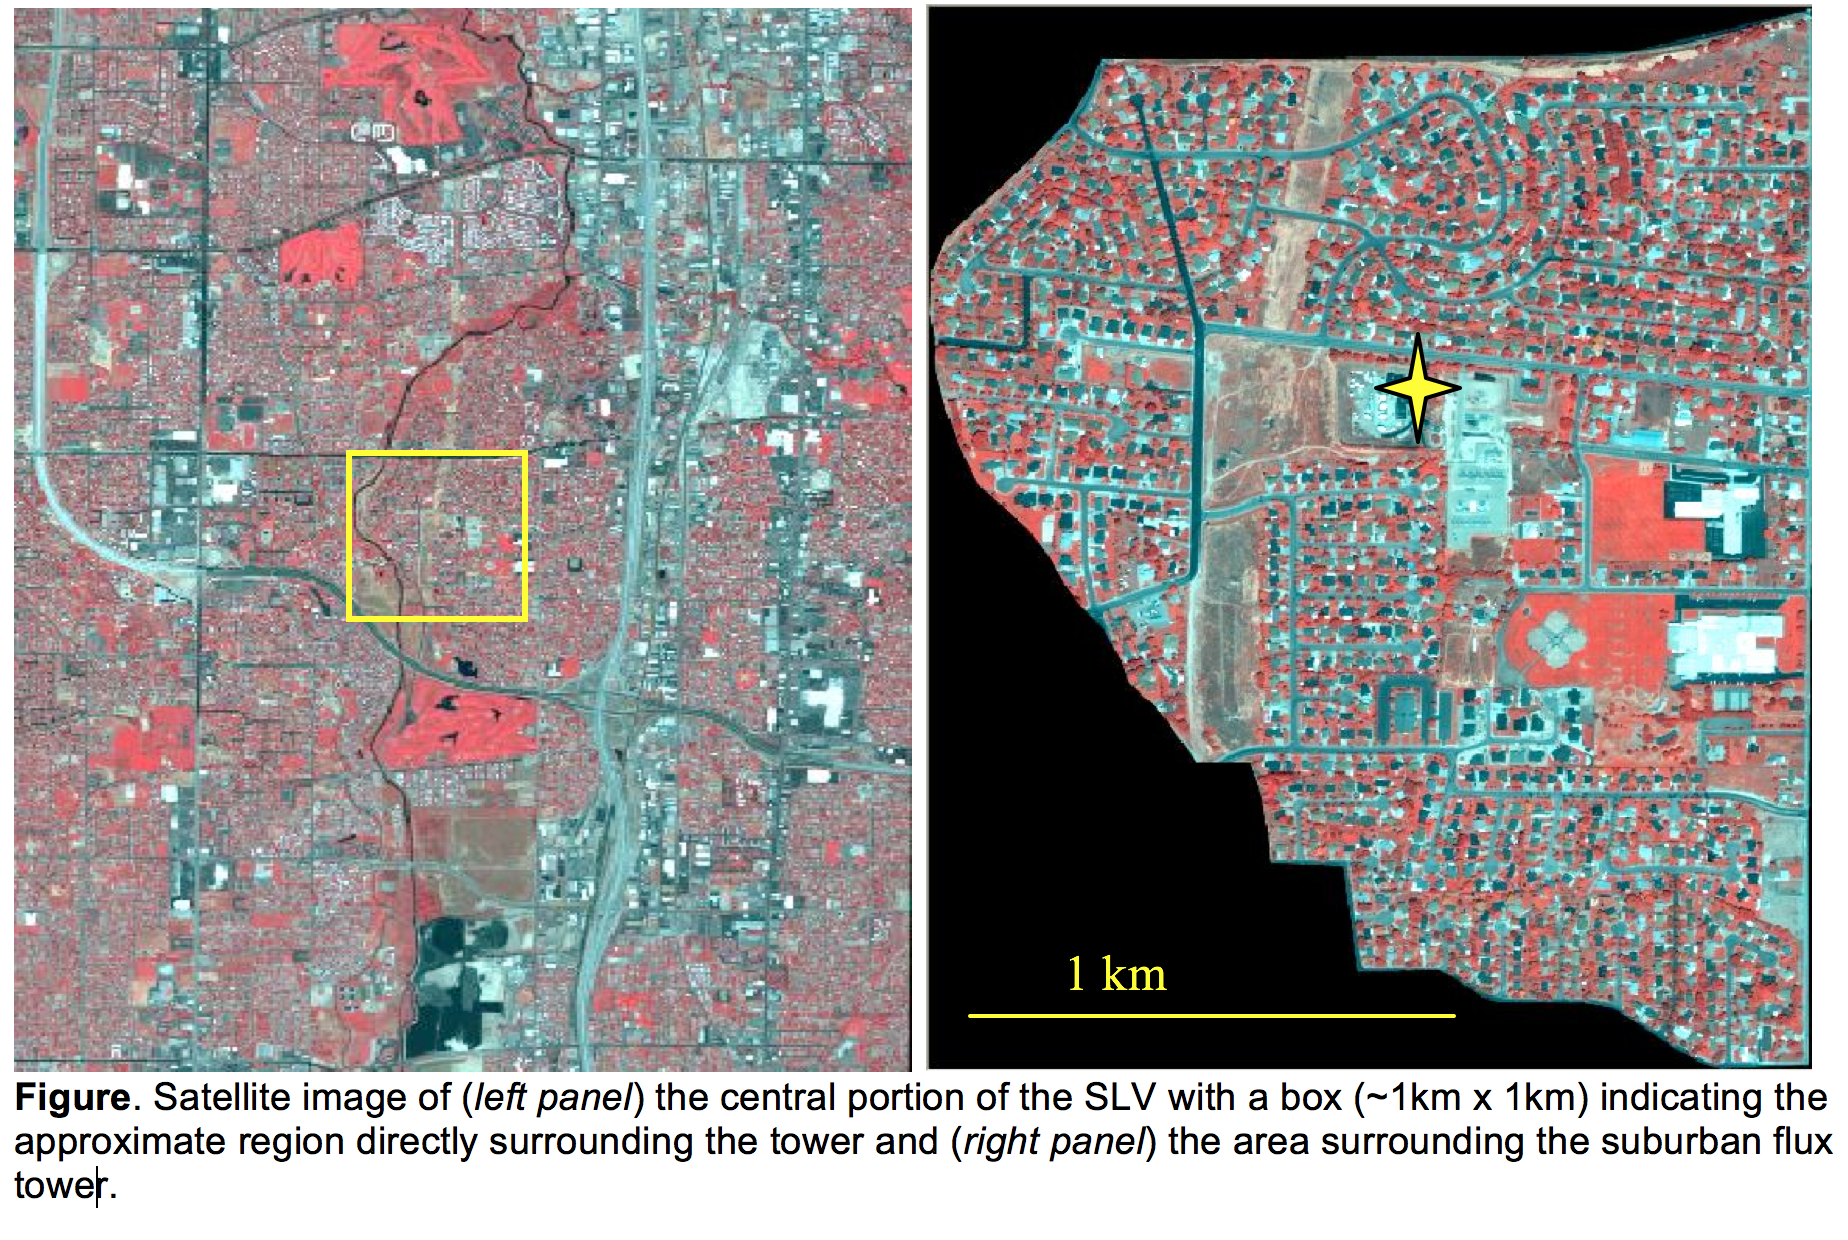
\includegraphics[width=1\textwidth]{fig1}
\end{figure}

\paragraph{\large Land Surface Cover Data, continued}~\\
\begin{figure}[H]
	\centering
	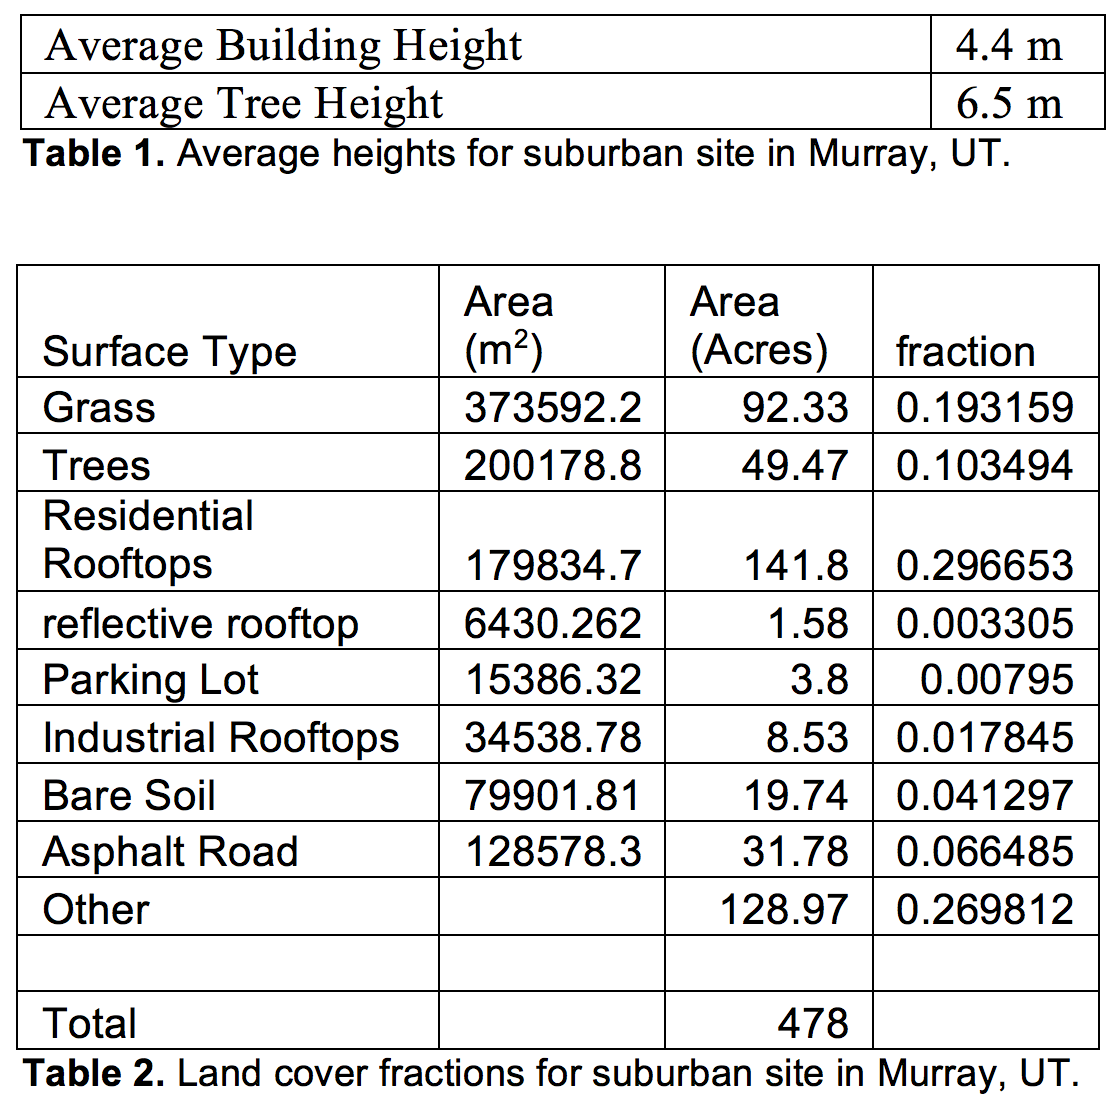
\includegraphics[width=0.5\textwidth]{fig2}
\end{figure}

\paragraph{\large Murray Tower Met and Flux Data}~\\
See Canvas or the course website for datasets and handouts.

\underline{Site Info}\\
Latitude: $40^\circ 39.11$ N, Longitude: $111^\circ 55.19$ W, Elevation: $1306\ \metre$, Average Site Albedo: $0.18$

Slope of the saturation vapor pressure temperature curve
$$\frac{de_s}{dT} \simeq \frac{L_v}{R_v}\frac{e_s}{T^2}$$

The psychrometric constant (Brunt 1952)
$$\gamma = \frac{c_p}{L_v}\frac{P}{\epsilon}$$

Where the latent heat of vaporization can be calculated as function of air temperature as (Stull, 1988)
$$L_v \simeq \left[2.501 - 0.00237 \cdot T(\celsius)\right]\times 10^6\ \joule\ \kilo\reciprocal\gram$$










\end{document}